\documentclass[11pt]{article}

\usepackage[margin=1in]{geometry}
\usepackage[T1]{fontenc}
\usepackage[utf8]{inputenc}
\usepackage{lmodern}
\usepackage{amsmath, amssymb, amsfonts}
\usepackage{booktabs}
\usepackage{multirow}
\usepackage{graphicx}
\usepackage{hyperref}
\usepackage{enumitem}
\usepackage{caption}
\usepackage{xcolor}
\usepackage{setspace}

\hypersetup{
    colorlinks=true,
    linkcolor=blue,
    citecolor=blue,
    urlcolor=blue
}

\title{Generative Trajectory Modeling for a 3-Link Planar Robotic Manipulator:\\
Comparing Deterministic Baselines, Conditional VAEs, and Diffusion Models}

\author{
    Student Name\\
    Department / University\\
    \texttt{student@email.edu}
    \and
    Advisor Name\\
    Department / University\\
    \texttt{advisor@email.edu}
}

\date{}

\begin{document}

\maketitle

\begin{abstract}
Trajectory generation for robotic manipulators is commonly formulated as a mapping from task-space motion requirements to joint-space trajectories. Even for low-degree-of-freedom systems, this mapping can be intrinsically one-to-many because multiple joint configurations can realize the same end-effector pose sequence. Deterministic regression models therefore face a structural limitation: they can recover a single representative trajectory, but they cannot naturally model the diversity of valid solutions. This work studies trajectory generation for a 3-link planar revolute manipulator as a conditional sequence generation problem. We build a reproducible research pipeline that includes analytical inverse kinematics, deterministic neural baselines (CNN, CNN+LSTM, CNN+GRU), a conditional variational autoencoder (cVAE), and a conditional diffusion model with DDPM/DDIM-style sampling. The dataset contains 27,000 trajectories across six geometric shape families, with a held-out hexagon split used for generalization analysis. The deterministic baselines achieve best validation losses of 0.0196 (CNN), 0.0054 (CNN+LSTM), and 0.0061 (CNN+GRU), while the cVAE attains a best validation reconstruction loss of 0.000774. On a completed 4,500-sample cVAE test run, the model achieves 0.0201 joint RMSE, 0.0291 end-effector position error, zero constraint violations, and 0.0154 joint RMSE on the held-out hexagon class. A conditional diffusion model is also implemented and trained to a best validation loss of 0.007965. Cross-model test-time comparison remains preliminary because the deterministic baselines and diffusion model are still summarized mainly through the earlier 6-sample stratified comparison artifact. These findings support the use of latent-variable generative models for manipulator trajectory generation, while also highlighting the importance of completing a uniform full-benchmark comparison across all model families.
\end{abstract}

\noindent\textbf{Keywords:} robotic manipulators, trajectory generation, inverse kinematics, conditional variational autoencoders, diffusion models, sequence modeling

\section{Introduction}

Trajectory generation is a core capability in robotic manipulation, motion planning, and autonomous control. For a manipulator to execute a desired end-effector path, the system must produce a smooth, feasible, and accurate joint-space trajectory that respects the robot kinematics and actuator limitations. Classical approaches address this problem using analytical inverse kinematics, optimization-based planners, or iterative numerical solvers. These methods are often highly accurate when the manipulator model is known, but they can become brittle under changing task requirements, repeated re-planning, or demands for real-time deployment.

Recent learning-based methods have shown that neural sequence models can learn inverse mappings directly from data, potentially amortizing the cost of trajectory inference. However, an important challenge remains under-emphasized in simple regression formulations: the mapping from task-space trajectories to joint-space trajectories is frequently one-to-many. Even in a planar manipulator, multiple inverse-kinematics branches can generate distinct but valid joint trajectories for the same end-effector path. A single deterministic regressor cannot explicitly represent this ambiguity and may instead collapse to one mode or average across modes.

This observation motivates the use of generative models for manipulator trajectory prediction. Rather than predicting one fixed trajectory, a generative model can represent a distribution over valid joint-space realizations conditioned on a task-space input. Such a formulation is attractive not only for accuracy, but also for downstream applications that benefit from diversity, such as energy-aware control, trajectory selection under secondary objectives, or deployment-time choice among feasible alternatives.

In this work, we study generative trajectory modeling for a 3-link planar robotic manipulator. The robot is intentionally simple enough to support analytical inverse kinematics and rigorous dataset generation, while still exhibiting the multi-solution structure needed to motivate generative learning. We compare deterministic baselines against two conditional generative model families: a conditional variational autoencoder (cVAE) with a latent trajectory representation, and a conditional diffusion model with iterative denoising and DDIM-based accelerated sampling.

\subsection*{Contributions}

The main contributions of the current work are:
\begin{enumerate}[leftmargin=1.5em]
    \item A reproducible end-to-end trajectory-generation pipeline for a 3-link planar manipulator, including analytical inverse kinematics, normalized dataset construction, and shape-based generalization splits.
    \item A controlled comparison between deterministic sequence regressors and generative trajectory models on the same manipulator task.
    \item A conditional VAE that substantially improves validation reconstruction error over deterministic baselines while enabling multi-sample joint-trajectory generation.
    \item A conditional diffusion implementation with 1D U-Net denoising, cosine noise scheduling, classifier-free guidance, and DDPM/DDIM sampling.
    \item A multi-metric evaluation framework covering reconstruction quality, task-space error, smoothness, energy proxy, diversity, and inference latency.
\end{enumerate}

\subsection*{Research Questions}

The current study is guided by three research questions that can already be grounded in the repository artifacts:
\begin{enumerate}[leftmargin=1.5em]
    \item \textbf{RQ1:} How far can deterministic neural baselines reduce trajectory-prediction error for a 3-link planar manipulator when conditioned on task-space waypoint sequences?
    \item \textbf{RQ2:} Does a conditional generative model, especially a cVAE, improve upon deterministic baselines while also supporting multi-sample trajectory generation for one-to-many inverse-kinematics mappings?
    \item \textbf{RQ3:} What do the currently completed results suggest about the trade-offs among accuracy, diversity, and inference cost when comparing deterministic, latent-variable, and diffusion-based approaches?
\end{enumerate}

\subsection*{Novelty and Scope}

The novelty of the current work lies less in proposing a fundamentally new generative architecture and more in building a controlled, reproducible comparison pipeline for one-to-many manipulator trajectory generation. In particular, the project combines analytical inverse kinematics, deterministic sequence baselines, a conditional VAE, a conditional diffusion model, shared normalization and evaluation infrastructure, and explicit generalization support through a held-out shape family. This makes the contribution valuable as an experimentally grounded benchmark-style study at the intersection of inverse kinematics and modern generative modeling, while keeping the paper's claims appropriately scoped to the completed evidence.

\subsection*{Paper Organization}

The remainder of the paper is organized as follows. Section 2 reviews relevant literature. Section 3 presents the robot model, kinematics, and dataset generation pipeline. Section 4 describes the deterministic and generative models. Section 5 details the training and evaluation protocol. Section 6 reports the currently available results. Section 7 discusses implications and the current status of the evaluation evidence. Section 8 summarizes the principal limitations. Section 9 outlines the most important future-work directions. Section 10 provides a reproducibility statement. Section 11 states data and code availability. Section 12 concludes the paper.

\section{Related Work}

Trajectory generation for manipulators has traditionally been approached through analytical inverse kinematics, sampling-based planning, and trajectory optimization. Optimization-based methods such as CHOMP, STOMP, and TrajOpt remain influential because they explicitly trade off smoothness, collision avoidance, and dynamic feasibility \cite{ratliff2009chomp, kalakrishnan2011stomp, schulman2013trajopt}. Their primary strength lies in geometric and physical interpretability; a recurring drawback is the computational burden associated with repeated optimization, especially when many similar queries must be answered online.

Learning-based inverse kinematics and motion generation methods attempt to amortize this computation by replacing iterative solving with direct prediction. Deterministic regressors can be highly efficient at inference time, but they remain limited when the output space is multi-modal. In inverse kinematics, this issue is fundamental: the same task-space target may admit multiple valid joint configurations, and an entire trajectory can often be realized by more than one branch-consistent joint sequence.

Latent-variable generative models provide one mechanism for addressing this ambiguity. Variational autoencoders, introduced in the deep latent-variable setting by Kingma and Welling \cite{kingma2013vae}, learn a structured latent space that supports sampling, interpolation, and conditional generation. Conditional latent-variable models have been used widely in trajectory prediction and robotics-related sequence generation, especially where multiple plausible futures or motion realizations exist.

Diffusion models provide a second route to generative modeling. Denoising Diffusion Probabilistic Models (DDPMs) \cite{ho2020ddpm} learn to reverse a stochastic noising process, while Denoising Diffusion Implicit Models (DDIMs) \cite{song2020ddim} provide a practical acceleration strategy at inference time. Classifier-free guidance \cite{ho2022cfg} enables conditional generation without a separate classifier and has become a standard conditioning mechanism.

Within robotics, diffusion-based generative modeling has gained traction through work such as Diffusion Policy \cite{chi2023diffusionpolicy}, which demonstrates strong performance for visuomotor policy learning, and Motion Planning Diffusion \cite{carvalho2023mpd}, which studies diffusion priors for robot motion planning. On the inverse-kinematics side, IKFlow \cite{ames2021ikflow} is especially relevant because it directly frames IK as a diverse generative modeling problem. These works collectively suggest that multimodal generative methods are well matched to robotics tasks where ambiguity and diversity matter.

The present work targets a narrower but experimentally useful gap: a controlled comparison of deterministic and generative trajectory models on a manipulator system with analytically verifiable kinematics, explicit multi-solution structure, and a reproducible data-generation pipeline.

\section{Robot Model and Dataset}

\subsection{Manipulator Definition}

The robot considered in this study is a 3-link planar revolute manipulator operating in the $xy$ plane. The link lengths are
\begin{equation}
    l_1 = 1.0,\quad l_2 = 1.0,\quad l_3 = 0.5,
\end{equation}
with joint limits
\begin{equation}
    q_i \in [-\pi, \pi], \quad i \in \{1,2,3\}.
\end{equation}
The manipulator base is fixed at the origin, and the end-effector pose is represented by $(x,y,\theta)$.
Figure~\ref{fig:arm_diagram} provides the geometric reference used throughout the remainder of the paper.

\begin{figure}[t]
\centering
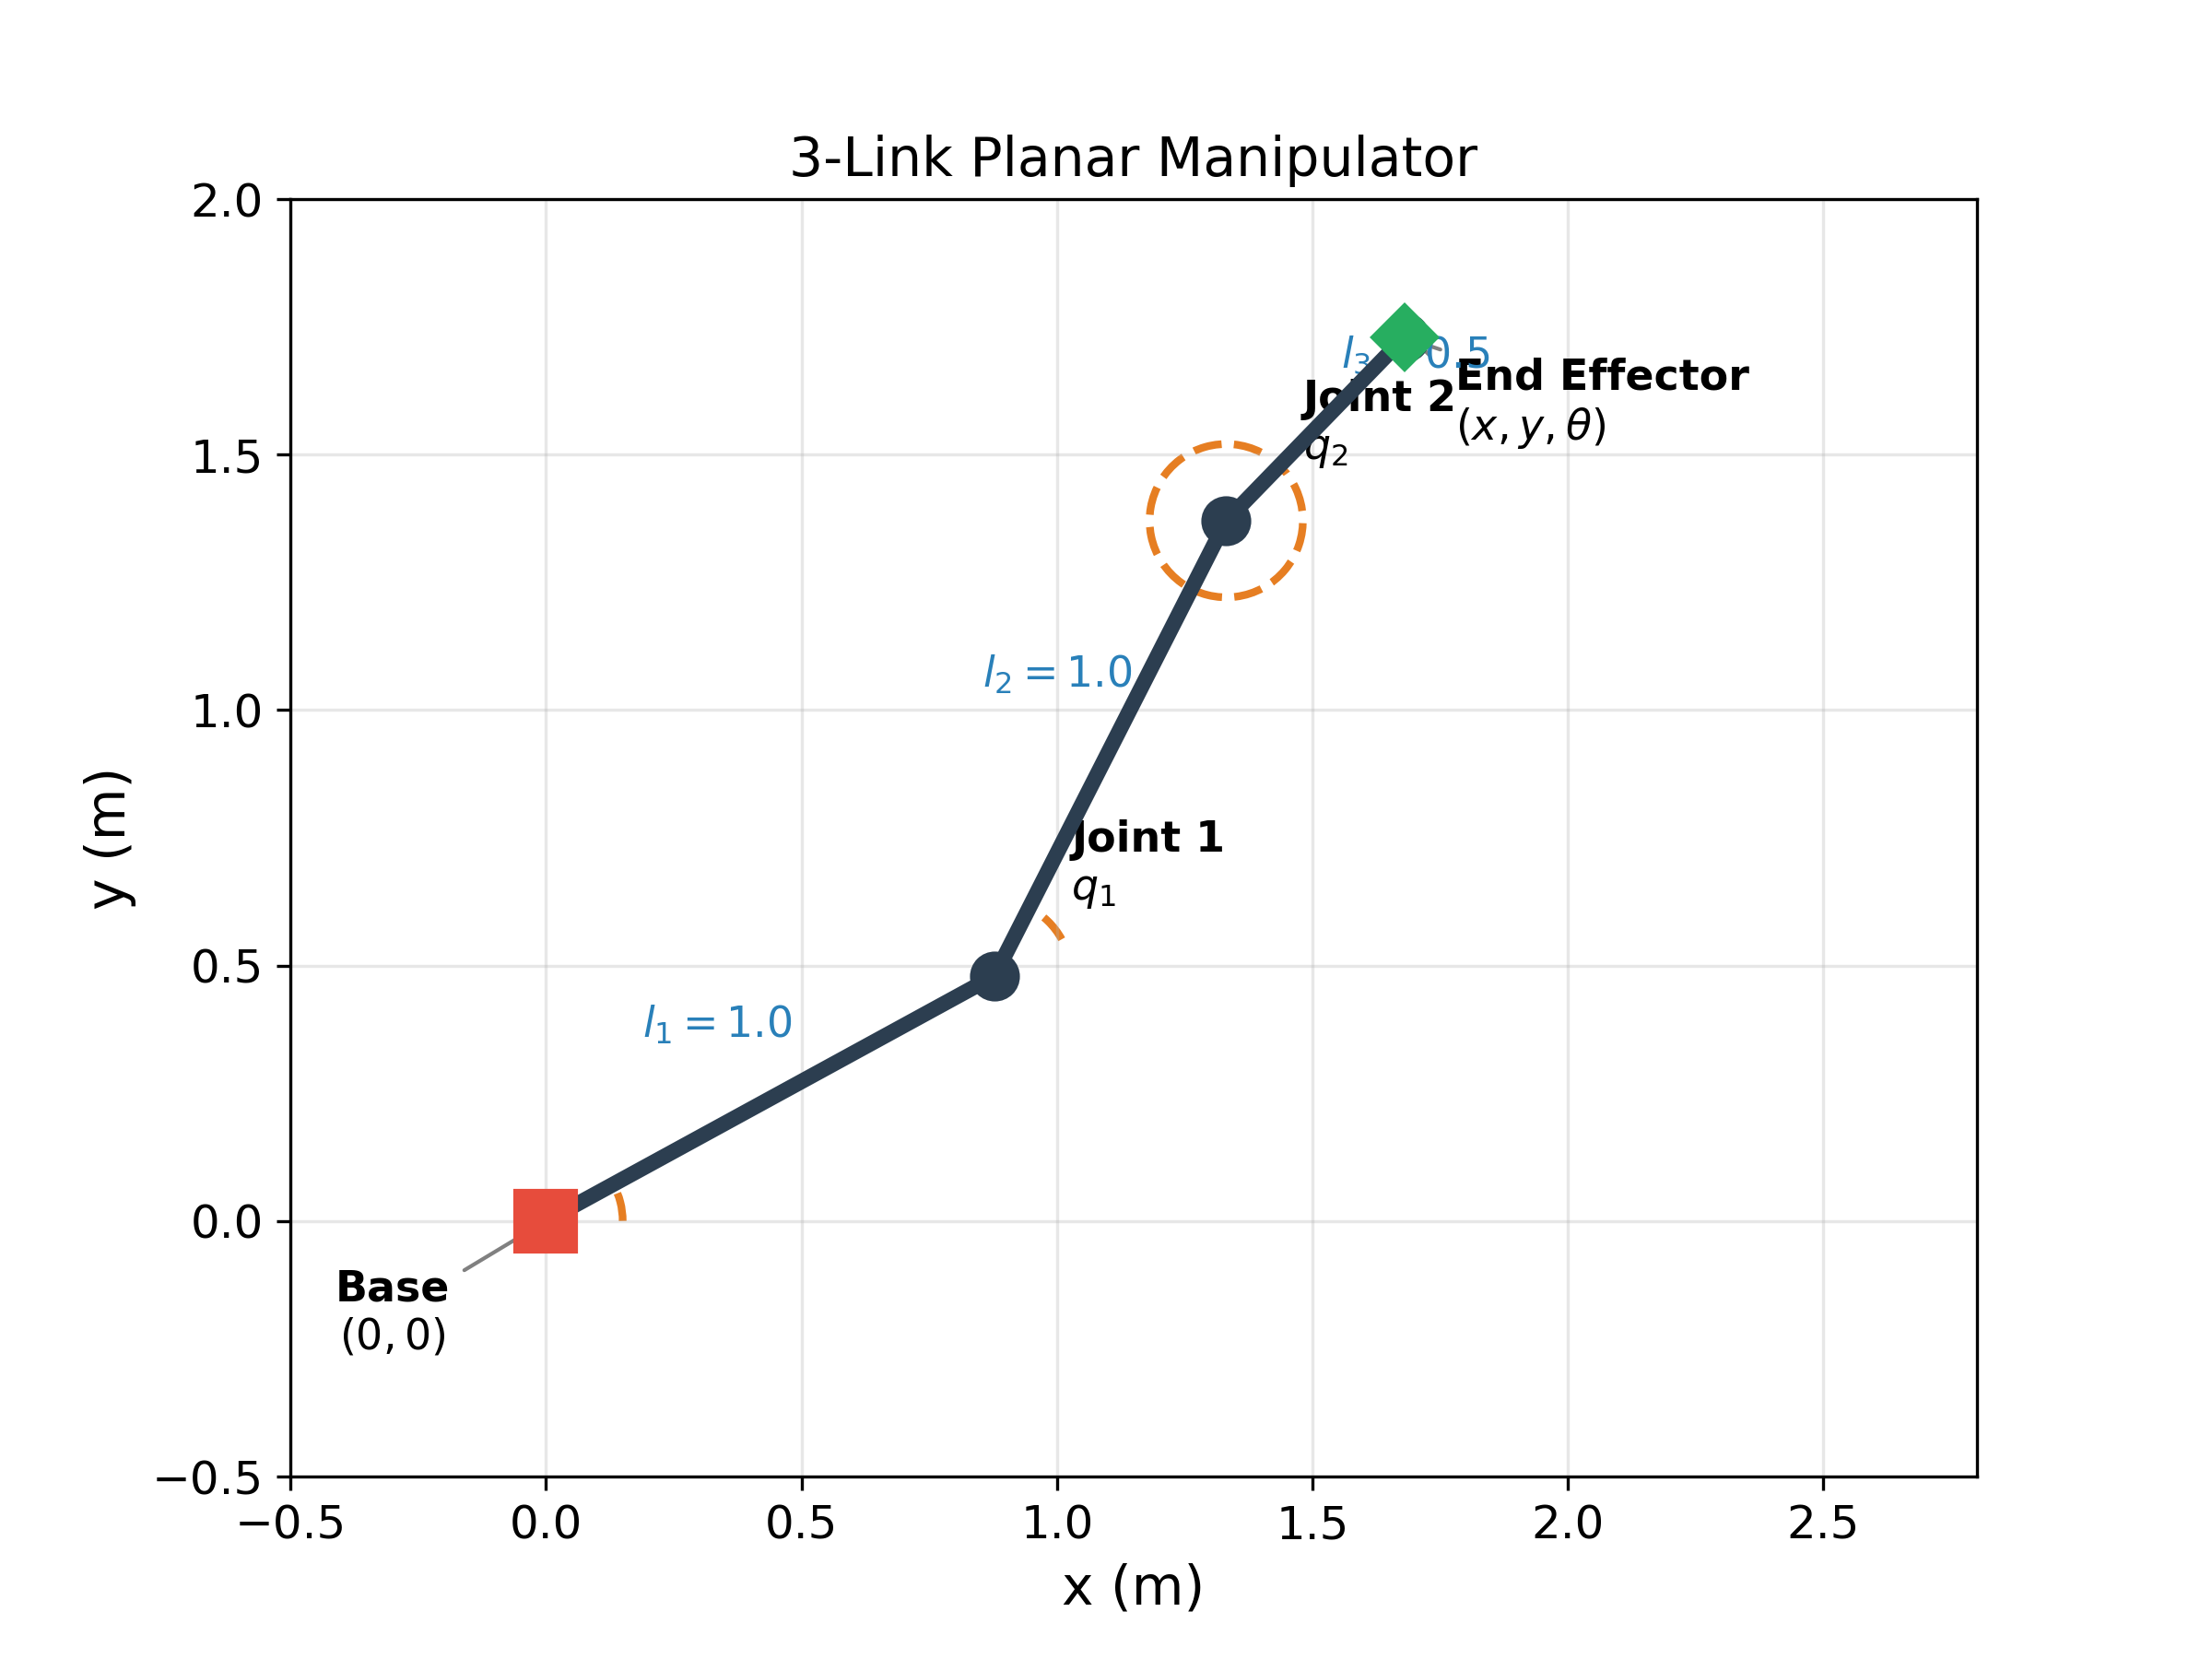
\includegraphics[width=0.62\linewidth]{../../figures/simulation/arm_diagram.png}
\caption{Geometry of the 3-link planar revolute manipulator used throughout the study. The system serves as the controlled testbed for comparing deterministic and generative trajectory models.}
\label{fig:arm_diagram}
\end{figure}

\subsection{Forward and Inverse Kinematics}

For joint configuration $\mathbf{q} = [q_1,q_2,q_3]^T$, the forward kinematics are
\begin{align}
    x &= l_1 \cos(q_1) + l_2 \cos(q_1+q_2) + l_3 \cos(q_1+q_2+q_3), \\
    y &= l_1 \sin(q_1) + l_2 \sin(q_1+q_2) + l_3 \sin(q_1+q_2+q_3), \\
    \theta &= q_1 + q_2 + q_3.
\end{align}

Inverse kinematics is solved analytically by first computing the wrist position and then solving the induced 2-link problem for the first two joints. In most reachable cases, this yields two valid branches (elbow-up and elbow-down), which makes the mapping from task-space trajectories to joint-space trajectories inherently multi-valued. Figure~\ref{fig:ik_branches} illustrates this branch ambiguity directly.

\begin{figure}[t]
\centering
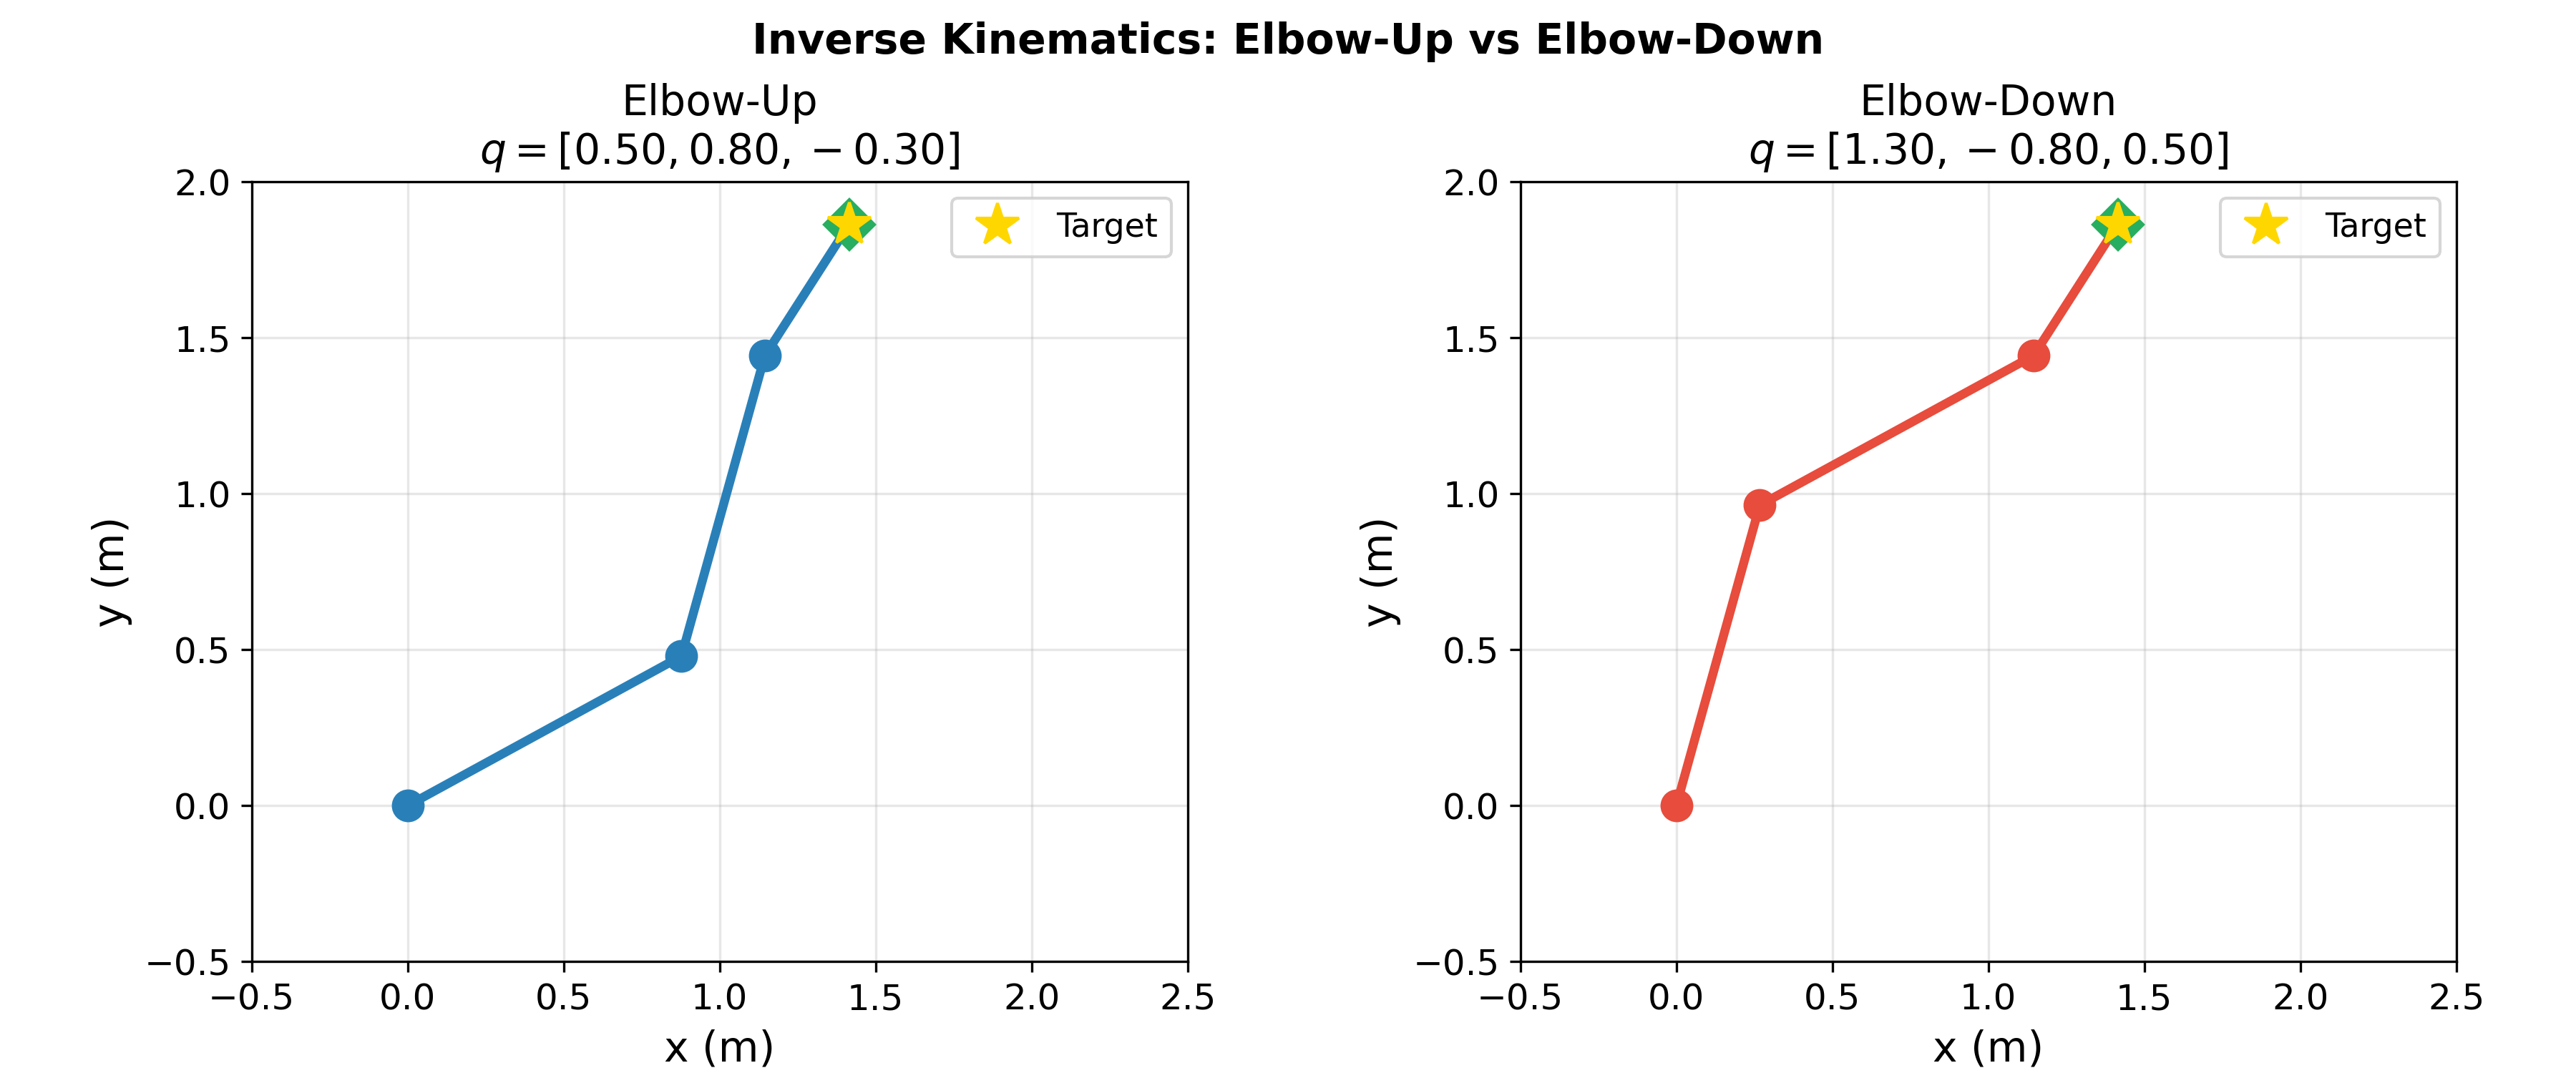
\includegraphics[width=0.72\linewidth]{../../figures/simulation/ik_branches.png}
\caption{Illustration of inverse-kinematics branch ambiguity in the planar manipulator. Multiple valid joint configurations can realize the same task-space sequence, motivating conditional generative modeling.}
\label{fig:ik_branches}
\end{figure}

\subsection{Trajectory Families and Dataset Split}

Six shape families are used to populate the dataset: circle, square, pentagon, hexagon, line, and random smooth trajectories. Each sample contains $T=100$ task-space waypoints and a corresponding joint-space trajectory.
Representative examples are shown in Figure~\ref{fig:shape_grid}.

The full dataset contains 27,000 trajectories:
\begin{itemize}[leftmargin=1.5em]
    \item 25,000 samples from five primary training shapes: circle, square, pentagon, line, and random smooth,
    \item 2,000 samples from hexagon reserved for test-time generalization.
\end{itemize}

The resulting split is shown in Table~\ref{tab:dataset_split}.

\begin{table}[h]
\centering
\caption{Dataset split used in the current project.}
\label{tab:dataset_split}
\begin{tabular}{lc}
\toprule
Split & Samples \\
\midrule
Train & 20,000 \\
Validation & 2,500 \\
Test & 4,500 \\
\bottomrule
\end{tabular}
\end{table}

\begin{figure}[t]
\centering
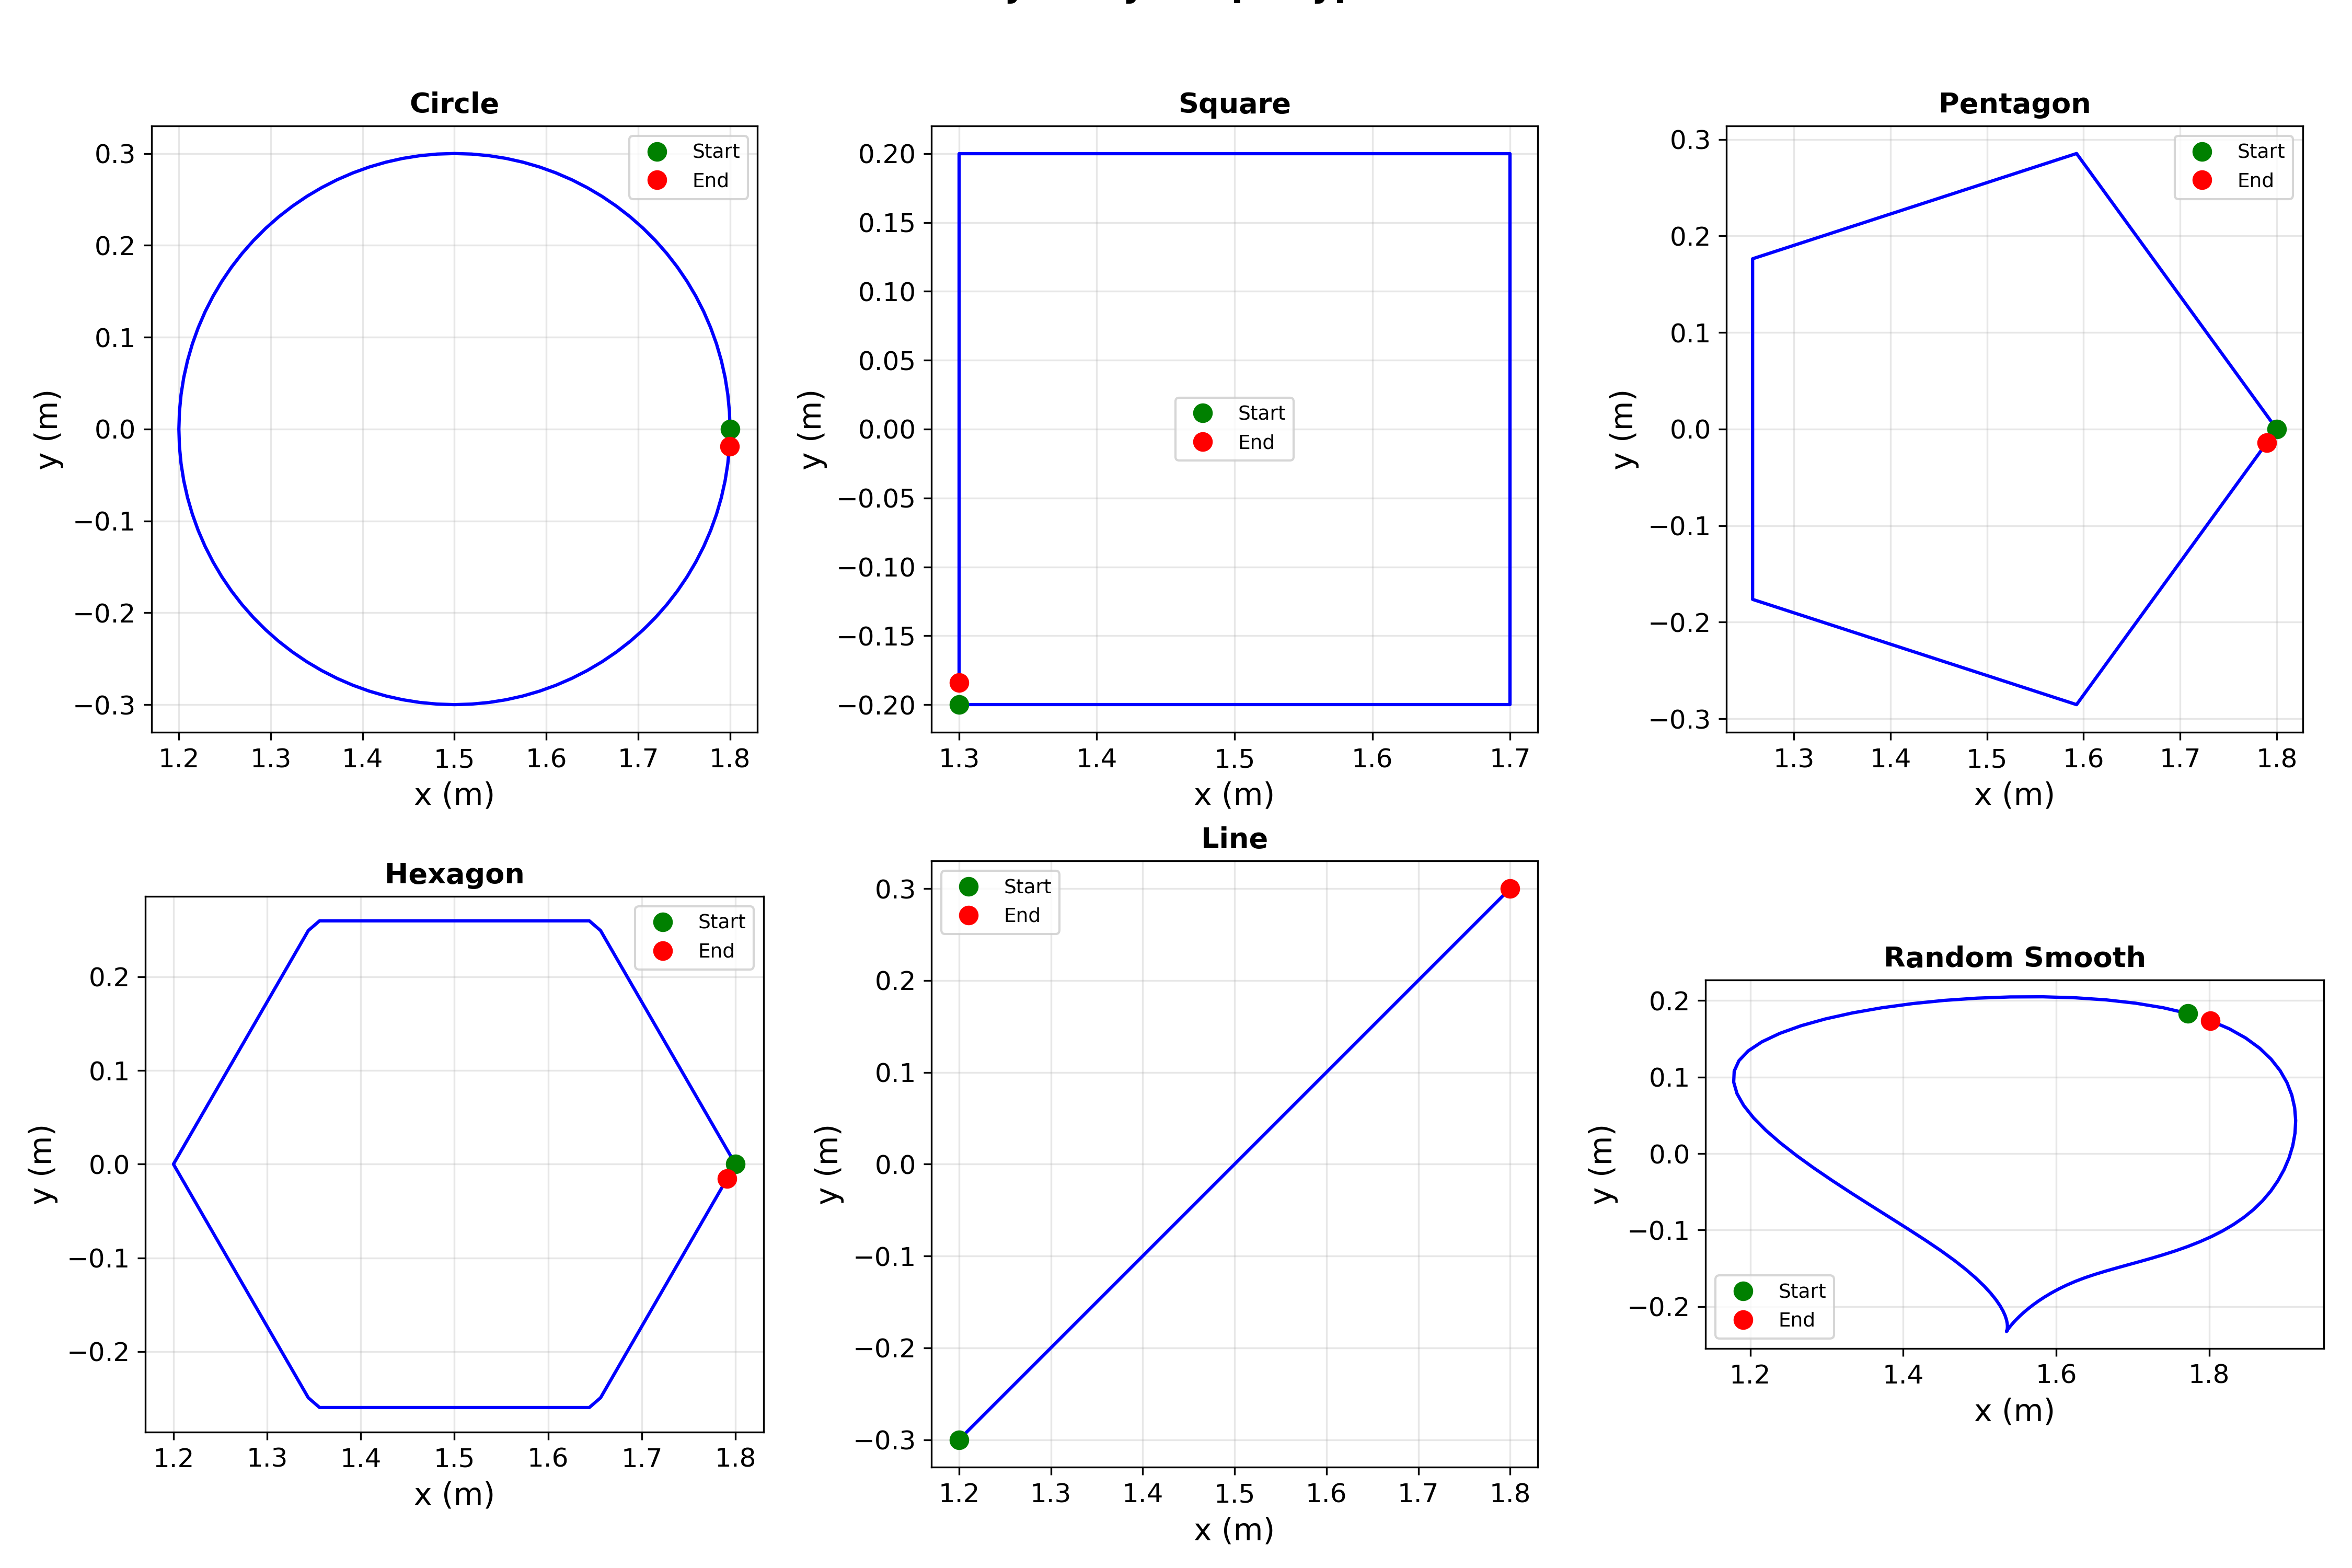
\includegraphics[width=0.82\linewidth]{../../figures/simulation/shape_trajectories_grid.png}
\caption{Representative task-space trajectory families used to build the dataset. The held-out hexagon family supports limited out-of-distribution generalization analysis.}
\label{fig:shape_grid}
\end{figure}

All task-space and joint-space trajectories are normalized using z-score statistics computed from the training set only.

\section{Methodology}

\subsection{Problem Formulation}

The learning problem is formulated as conditional sequence generation:
\begin{equation}
    f_\theta : \mathbf{W} \in \mathbb{R}^{100 \times 3} \rightarrow \mathbf{Q} \in \mathbb{R}^{100 \times 3},
\end{equation}
where $\mathbf{W}$ is the task-space waypoint sequence and $\mathbf{Q}$ is the joint-space trajectory. Deterministic models learn a direct mapping from $\mathbf{W}$ to one predicted $\mathbf{Q}$, whereas generative models instead learn a conditional distribution $p(\mathbf{Q}\mid\mathbf{W})$.

\subsubsection{Notation}

Throughout the paper, $\mathbf{W}$ denotes a task-space waypoint sequence of length $T=100$, $\mathbf{Q}$ denotes the corresponding joint-space trajectory, and $z$ denotes a latent variable used by the cVAE. For stochastic models, $K$ denotes the number of generated samples used during evaluation when computing oracle or mean-sample metrics.

\subsubsection{Reference Analytical IK Baseline}

In addition to learned models, the project includes an analytical inverse-kinematics reference solver. This method is not treated as a learned competitor; instead, it serves as a kinematics-grounded reference point for evaluating how closely the learned models approach branch-consistent trajectory reconstruction on the synthetic dataset. In the current subset comparison artifact, the analytical IK method produces near-zero geometric errors, which is expected because the dataset itself is generated from the same kinematic structure.

\subsection{Deterministic Baselines}

Three deterministic baselines are implemented:
\begin{enumerate}[leftmargin=1.5em]
    \item \textbf{CNN:} a temporal convolutional regressor with global pooling and a fully connected decoder,
    \item \textbf{CNN+LSTM:} a convolutional encoder followed by a two-layer LSTM decoder,
    \item \textbf{CNN+GRU:} a convolutional encoder followed by a two-layer GRU decoder.
\end{enumerate}

\subsection{Conditional Variational Autoencoder}

The cVAE is the primary generative baseline in the current study. It consists of
\begin{enumerate}[leftmargin=1.5em]
    \item a 1D-CNN condition encoder that maps task-space waypoints to a 64-dimensional embedding,
    \item a bidirectional GRU encoder that predicts the latent mean and log-variance,
    \item a GRU decoder that reconstructs the joint-space trajectory from the latent code and condition embedding.
\end{enumerate}

The trained configuration uses a latent dimension of 16 and contains 637,350 trainable parameters.

Training minimizes a weighted combination of reconstruction error, KL divergence, an energy proxy, and a smoothness penalty:
\begin{equation}
    \mathcal{L} =
    \lambda_{\text{recon}}\mathcal{L}_{\text{recon}}
    + \beta(t)D_{KL}
    + \lambda_{\text{energy}}\mathcal{L}_{\text{energy}}
    + \lambda_{\text{smooth}}\mathcal{L}_{\text{smooth}}.
\end{equation}

KL annealing is implemented using a cyclical schedule with warmup to avoid posterior collapse while preserving a meaningful latent structure.

\subsection{Conditional Diffusion Model}

The second generative model is a conditional diffusion model using
\begin{enumerate}[leftmargin=1.5em]
    \item a 1D-CNN condition encoder,
    \item a 1D U-Net denoiser,
    \item sinusoidal time embeddings,
    \item classifier-free guidance during inference.
\end{enumerate}

The current trained model has 1,425,606 trainable parameters. The forward process uses a cosine noise schedule with 1,000 diffusion steps. During inference, both DDPM and DDIM sampling are implemented, though DDIM is the practical default due to lower runtime cost.

\subsection{Model Summary}

Table~\ref{tab:model_summary} summarizes the principal model families currently implemented in the project.

\begin{table}[h]
\centering
\caption{Model families currently implemented in the project.}
\label{tab:model_summary}
\begin{tabular}{lccc}
\toprule
Model & Type & Parameters & Inference Style \\
\midrule
CNN & Deterministic & 140,588 & one-shot regression \\
CNN+LSTM & Deterministic & 246,787 & one-shot recurrent decoding \\
CNN+GRU & Deterministic & 188,931 & one-shot recurrent decoding \\
cVAE & Generative & 637,350 & latent sampling + decode \\
Diffusion & Generative & 1,425,606 & iterative denoising \\
\bottomrule
\end{tabular}
\end{table}

\section{Training and Evaluation Protocol}

\subsection{Training Setup}

All models are trained on normalized trajectories with fixed random seeds and gradient-based optimization. The deterministic baselines use Adam with a learning rate of 0.001. The cVAE uses Adam with a learning rate of 0.0003, batch size 64, and cyclical KL annealing. The diffusion model uses AdamW with a learning rate of 0.0002, a cosine beta schedule, and EMA tracking.

\subsection{Experimental Configuration}

The main training configurations used by the learned models are summarized in Table~\ref{tab:training_config}. These settings reflect the values currently implemented and logged in the project artifacts.

\begin{table}[h]
\centering
\caption{Training configurations of the principal learned models.}
\label{tab:training_config}
\begin{tabular}{lcccc}
\toprule
Model & Optimizer & LR & Batch Size & Max Epochs \\
\midrule
CNN / CNN+LSTM / CNN+GRU & Adam & 0.001 & 64 & 200 \\
cVAE & Adam & 0.0003 & 64 & 500 \\
Diffusion & AdamW & 0.0002 & 64 & 500 \\
\bottomrule
\end{tabular}
\end{table}

\subsection{Metrics}

The current evaluation framework computes:
\begin{enumerate}[leftmargin=1.5em]
    \item joint-space RMSE,
    \item end-effector position error,
    \item end-effector orientation error,
    \item path tracking error,
    \item energy proxy,
    \item smoothness (jerk-based),
    \item inference latency,
    \item diversity score for stochastic models,
    \item constraint violation rate.
\end{enumerate}

For generative models, the framework reports both oracle metrics (best sample among $K$ generated trajectories per condition) and mean sample metrics (average quality across the $K$ generated samples).

The principal metrics used in the current comparison pipeline are defined as follows. Joint-space accuracy is measured with root-mean-squared error,
\begin{equation}
    \mathrm{RMSE}(\hat{\mathbf{Q}}, \mathbf{Q})
    =
    \sqrt{\frac{1}{3T}\sum_{t=1}^{T}\|\hat{\mathbf{q}}_t - \mathbf{q}_t\|_2^2 }.
\end{equation}
End-effector position error is computed as the mean Euclidean distance between predicted and reference task-space positions after forward kinematics, while orientation error is the mean absolute wrapped angular difference over the full trajectory. Path-tracking error is computed with dynamic time warping in the current evaluation code, normalized by trajectory length.

The energy proxy reported in the present comparison uses the mean squared joint-velocity magnitude,
\begin{equation}
    \mathcal{E}_{\mathrm{vel}}
    =
    \frac{1}{T-1}\sum_{t=1}^{T-1}\|\mathbf{q}_{t+1} - \mathbf{q}_t\|_2^2,
\end{equation}
while smoothness is quantified through the mean squared jerk magnitude obtained by finite differences. Inference latency is reported as the median runtime over repeated forward passes. For stochastic models, diversity is measured as the mean pairwise path-tracking distance between generated samples, and joint-limit feasibility is summarized through the fraction of joint values that violate the allowed range.

\subsection{Current Evaluation Status}

The evaluation pipeline is implemented and now supports two completed evidence layers: a full 4,500-sample cVAE evaluation executed through the standalone external-GPU notebook workflow, and an earlier 6-sample stratified cross-model comparison containing one example from each test-set shape class. The cVAE therefore now has full-test evidence, but model-to-model ranking across all learned methods should still be treated as provisional until the deterministic baselines and diffusion model are evaluated under the same full protocol.

\subsection{Generalization Protocol}

Generalization is probed through the dataset split itself: the test set contains both in-distribution samples and trajectories from a held-out hexagon shape family that is not used during training. This gives the project two complementary evaluation views, namely interpolation across seen shape families and limited out-of-distribution assessment on unseen geometry. The completed full cVAE artifact retains this split structure and reports strong held-out hexagon behavior, while the broader cross-model comparison still relies on the earlier subset artifact.

\subsection{Generative Evaluation Protocol}

For generative models, the current evaluation pipeline draws $K=10$ samples per conditioning input and reports both oracle and mean-sample behavior. In the completed implementation, oracle selection is based on the lowest joint-space RMSE among the sampled trajectories, while diversity is computed as the mean pairwise dynamic-time-warping distance between generated samples. To support downstream analysis, the pipeline can cache the full set of generated samples for each evaluated condition rather than only the oracle trajectory.

Inference latency is benchmarked separately from per-sample metric accumulation. The current implementation measures latency on a small stratified subset of conditions, uses repeated forward passes per condition, reports the median latency for each condition, and then averages those per-condition medians into the model-level latency number shown in the summary tables. This avoids conflating raw model runtime with dataset traversal overhead.

Table~\ref{tab:eval_protocol} summarizes the principal evaluation settings reflected in the current code and completed artifacts.

\begin{table}[h]
\centering
\caption{Evaluation protocol settings reflected in the implemented pipeline and the currently completed artifacts.}
\label{tab:eval_protocol}
\begin{tabular}{p{5.2cm}p{8.6cm}}
\toprule
Setting & Current Value / Behavior \\
\midrule
Completed cVAE artifact size & 4,500 test samples \\
Completed cross-model artifact size & 6 stratified test samples \\
Completed shape coverage in cross-model artifact & 1 sample each from circle, square, pentagon, hexagon, line, and random\_smooth \\
Generative samples per condition & $K=10$ \\
Oracle selection rule & Lowest joint-space RMSE among generated samples \\
Path-tracking metric & DTW-based distance \\
Diversity metric & Mean pairwise DTW distance across generated samples \\
Latency benchmarking & 10 repeated runs on 3 stratified conditions, aggregated as mean of per-condition medians \\
Generative cache behavior & Full generated sample set stored for each evaluated condition \\
Included models in current configuration & analytical\_ik, CNN, CNN+LSTM, CNN+GRU, cVAE, diffusion\_ddim \\
\bottomrule
\end{tabular}
\end{table}

\subsection{Statistical Reporting Conventions}

The current manuscript reports validation losses from the best logged checkpoints of the completed training runs, full-test cVAE metrics from the integrated 4,500-sample artifact, and cross-model evaluation metrics from the earlier stratified subset artifact. These numbers are therefore best interpreted as reproducible descriptive results from the present repository state, not as final multi-seed inferential estimates. Formal statistical comparisons, confidence intervals, and multi-seed significance analysis are intentionally deferred until the uniform full benchmark and ablation phases are completed.

\subsection{Reproducibility and Artifact Availability}

The present study is built around a reproducible codebase with modular simulation, training, and evaluation components. Current repository artifacts include:
\begin{enumerate}[leftmargin=1.5em]
    \item dataset generation and normalization code,
    \item trained checkpoints for deterministic, cVAE, and diffusion models,
    \item evaluation scripts and summary reports,
    \item paper and thesis drafting material.
\end{enumerate}

In addition, a standalone self-contained notebook has been prepared for portable cVAE training and evaluation on an external GPU environment. This notebook has now been used to complete the full-scale 4,500-sample cVAE evaluation without requiring direct dependency on the local repository structure, and it remains the recommended path for larger external-GPU reruns.

\section{Results}

\subsection{Training Outcome Summary}

Before examining each model family in detail, Table~\ref{tab:training_outcomes} summarizes the principal completed training outcomes across all learned models. This table is intended as a compact overview of scale, convergence point, and validation statistic. The diffusion validation objective should still be interpreted separately from deterministic or cVAE reconstruction losses.

\begin{table}[h]
\centering
\caption{Summary of completed training outcomes across learned models.}
\label{tab:training_outcomes}
\begin{tabular}{p{2.1cm}p{2.0cm}p{2.9cm}p{2.4cm}p{4.3cm}}
\toprule
Model & Parameters & Best Validation Statistic & Best Epoch / Logged Epochs & Interpretation \\
\midrule
CNN & 140,588 & 0.0196 & 131 / 161 & Deterministic regression baseline \\
CNN+LSTM & 246,787 & 0.0054 & 53 / 83 & Strongest deterministic baseline \\
CNN+GRU & 188,931 & 0.0061 & 26 / 56 & Recurrent baseline slightly behind LSTM \\
cVAE & 637,350 & 0.000774 (reconstruction) & 426 / 486 & Best reconstruction-oriented learned result and current strongest full-test generative artifact \\
Diffusion & 1,425,606 & 0.007965 (diffusion loss) & 414 / 494 & Stable training, but objective not directly comparable to cVAE reconstruction loss \\
\bottomrule
\end{tabular}
\end{table}

\subsection{Analytical IK Reference}

The evaluation pipeline includes an analytical inverse-kinematics reference method as a non-learned comparator. On the completed subset artifact, this reference yields effectively zero geometric reconstruction and tracking error, which is expected in the current synthetic setting because the dataset is derived from the same kinematic model. Its main role in the paper is therefore interpretive: it provides a reference ceiling for what the learned models are trying to approximate under branch-consistent trajectory generation.

\subsection{Deterministic Baselines}

The current best validation losses for the deterministic baselines are shown in Table~\ref{tab:baseline_results}.

\begin{table}[h]
\centering
\caption{Best validation losses for deterministic baselines.}
\label{tab:baseline_results}
\begin{tabular}{lcc}
\toprule
Model & Best Validation Loss & Best-Epoch Index in Logged History \\
\midrule
CNN & 0.0196 & 131 / 161 \\
CNN+LSTM & \textbf{0.0054} & 53 / 83 \\
CNN+GRU & 0.0061 & 26 / 56 \\
\bottomrule
\end{tabular}
\end{table}

These results show a clear gain from temporal modeling. The recurrent baselines outperform the pure CNN by roughly a factor of three to four, indicating that sequence structure matters strongly in this task. The convergence behavior is also visually clear in Figure~\ref{fig:baseline_curves}.

The broader evaluation pipeline also reports an analytical inverse-kinematics reference method when test-time artifacts are available. That reference should be interpreted as a kinematic ceiling for this controlled synthetic setting rather than as a directly comparable learned baseline.

\begin{figure}[t]
\centering
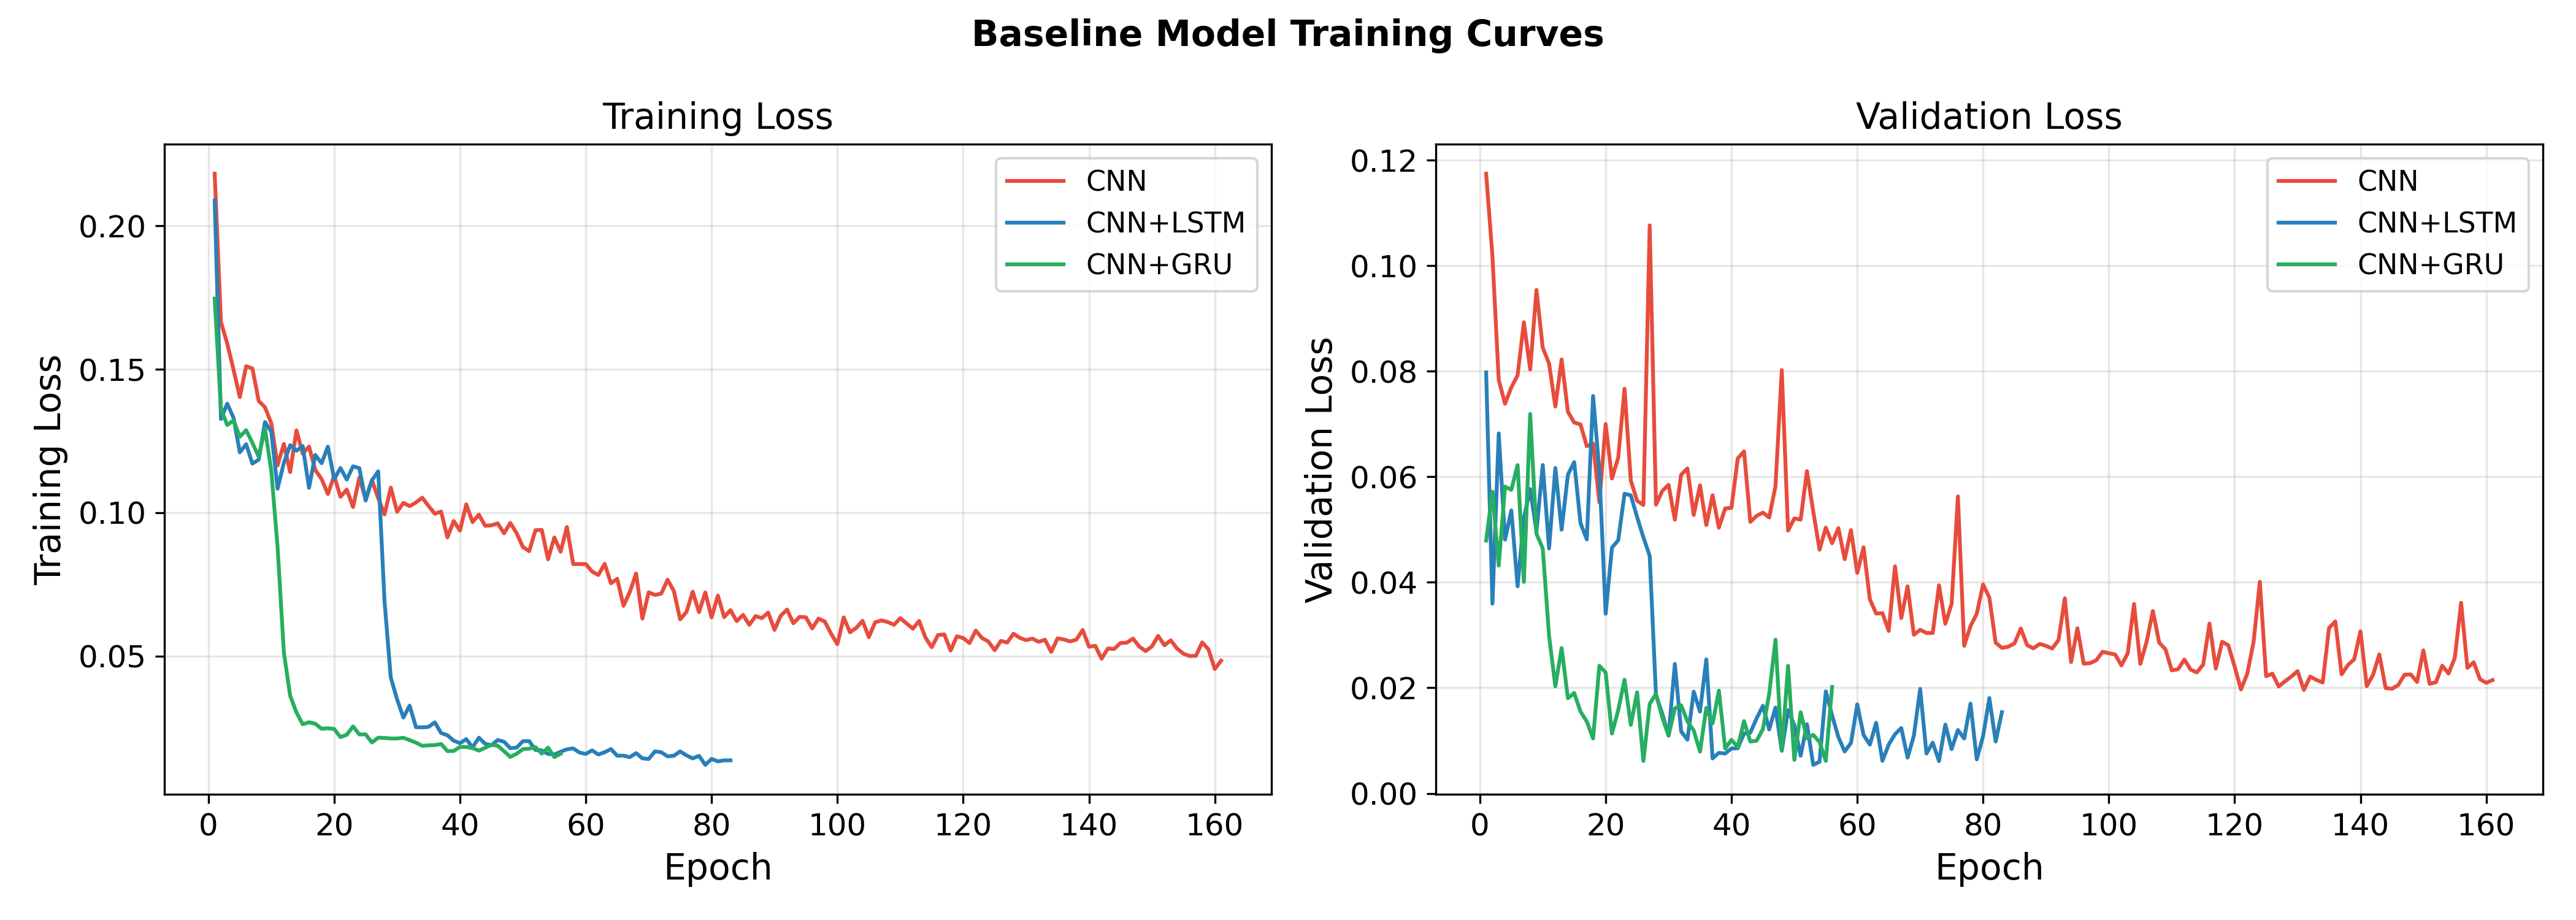
\includegraphics[width=0.82\linewidth]{../../figures/baselines/training_curves.png}
\caption{Training and validation loss curves for the deterministic baselines. Recurrent decoders converge to substantially lower validation loss than the pure CNN regressor.}
\label{fig:baseline_curves}
\end{figure}

\subsection{cVAE Performance}

The cVAE now reaches a best validation reconstruction loss of 0.000774 at epoch 426 and runs for 486 logged epochs before early termination. Relative to the strongest deterministic baseline (CNN+LSTM), this corresponds to a 6.98$\times$ reduction in validation reconstruction loss. The latent regularization remains healthy: the KL term stays non-zero throughout training and is approximately 0.028 at the best validation-reconstruction epoch, suggesting that the model avoids posterior collapse and uses the latent variable meaningfully. Qualitative reconstruction behavior is shown in Figure~\ref{fig:cvae_recon}, while Figure~\ref{fig:cvae_latent} provides a qualitative view of the learned latent organization.

The strongest new evidence comes from the completed 4,500-sample cVAE test evaluation. On that run, the cVAE achieves 0.02012 joint RMSE, 0.02911 end-effector position error, 0.01493 end-effector orientation error, 0.02882 path-tracking error, 0.000427 energy proxy, $9.10\times10^{-6}$ smoothness jerk, and 0.0 constraint-violation rate. The diversity score is 0.02157 in the current evaluation implementation. The oracle-versus-mean-sample gap is also informative: mean-sample joint RMSE is 0.03436, while oracle selection reduces this to 0.02012, a 41.43\% improvement. This confirms that the model is generating multiple distinct candidates and that a downstream selector could exploit that diversity.

Per-shape results show the strongest cVAE performance on pentagon (0.01311 joint RMSE), circle (0.01420), square (0.01465), and the held-out hexagon class (0.01543). Line trajectories are moderately harder at 0.02245, while random\_smooth trajectories remain the clearest error concentration at 0.05495. The held-out hexagon result is especially important because that shape family is excluded from training, suggesting that the cVAE learns a trajectory prior that generalizes beyond memorized training geometry.

In terms of model scale, the cVAE is noticeably larger than the deterministic baselines but remains below one million trainable parameters. This places it in a practical middle ground: expressive enough to capture multimodal behavior, yet still compact enough to remain plausible for repeated experimentation and downstream deployment-oriented studies.

\begin{figure}[t]
\centering
\includegraphics[width=0.84\linewidth]{../../results/plots/cvae_full_4500_reconstruction_samples.png}
\caption{Example cVAE reconstructions from the integrated full-scale run. The model recovers smooth joint-space sequences while preserving the structure of the conditioning signal.}
\label{fig:cvae_recon}
\end{figure}

\begin{figure}[t]
\centering
\includegraphics[width=0.74\linewidth]{../../results/plots/cvae_full_4500_latent_tsne.png}
\caption{Two-dimensional visualization of the learned cVAE latent representation from the full-scale run. The latent organization provides qualitative support for meaningful structured variation in the learned trajectory space.}
\label{fig:cvae_latent}
\end{figure}

\subsection{Diffusion Training Performance}

The diffusion model reaches a best validation loss of 0.007965 at epoch 414 with 494 logged epochs. This demonstrates successful training convergence and confirms that the conditioning and denoising pipeline is operational. However, the diffusion validation objective is not directly comparable to the cVAE reconstruction objective and should therefore be interpreted primarily as evidence of stable training. Figure~\ref{fig:diffusion_denoising} illustrates the iterative refinement process learned by the denoiser.

The diffusion network is also the largest learned model in the repository at 1.43M parameters. Even before full-scale inference benchmarking, this already foreshadows a central trade-off in the project: diffusion offers a flexible generative formulation, but likely at a higher runtime and systems cost than latent-variable alternatives such as the cVAE.

\begin{figure}[t]
\centering
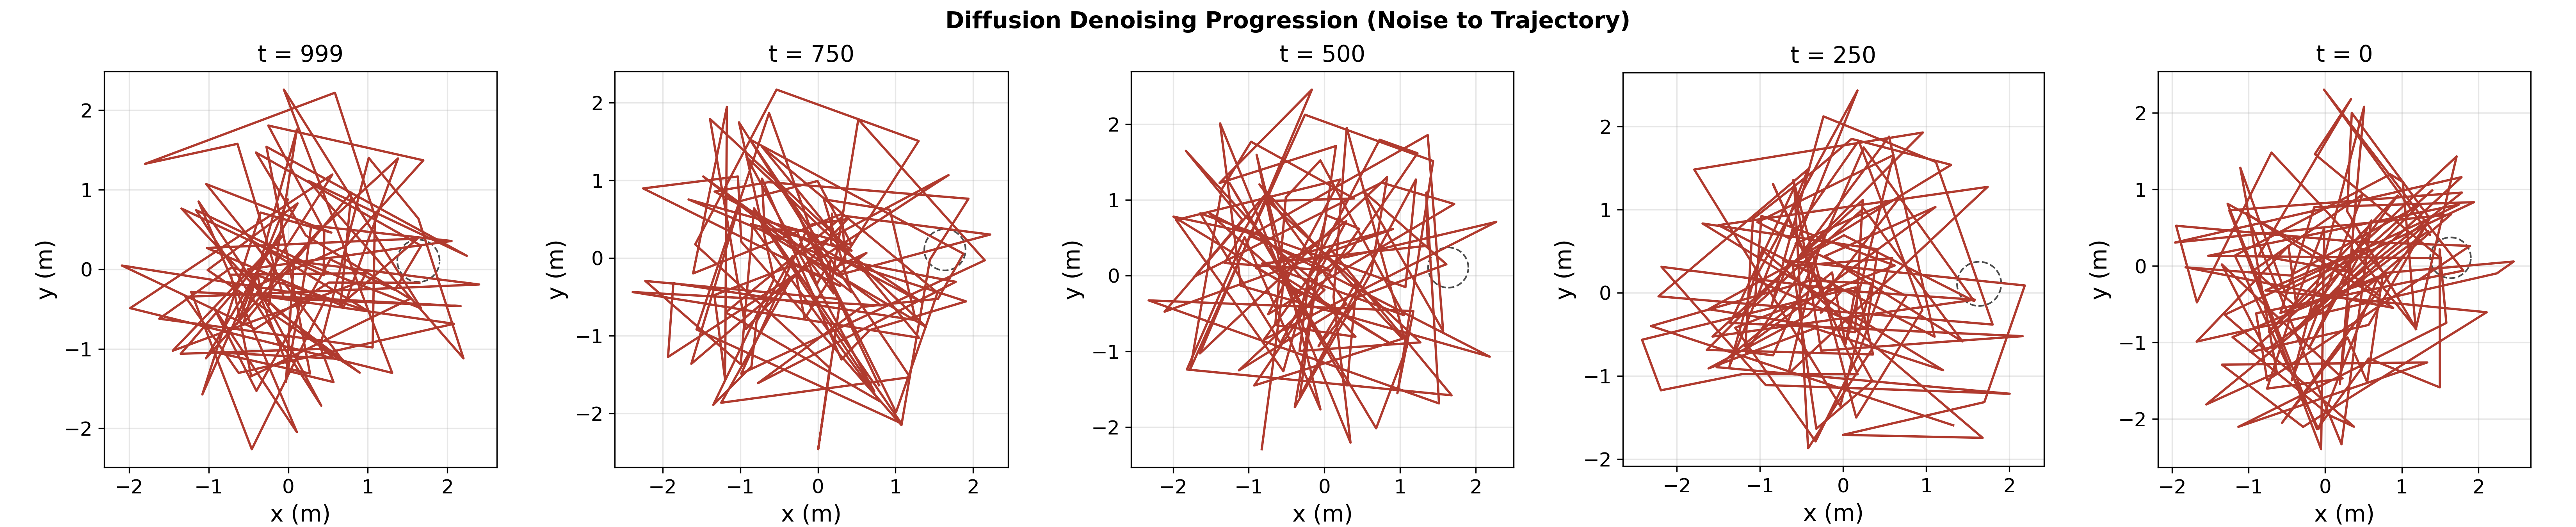
\includegraphics[width=0.84\linewidth]{../../figures/diffusion/denoising_progression.png}
\caption{Progressive denoising behavior of the conditional diffusion model. Starting from noise, the model iteratively refines the sample toward a structured joint-space trajectory.}
\label{fig:diffusion_denoising}
\end{figure}

\subsection{Preliminary Comparative Evaluation}

The completed subset-level evaluation currently yields the metrics shown in Table~\ref{tab:subset_eval}.

\begin{table}[p]
\centering
\caption{Preliminary subset evaluation on 6 stratified test samples.}
\label{tab:subset_eval}
\begin{tabular}{lcccccccc}
\toprule
Model & RMSE & EE Pos & EE Ori & Path & Energy & Smooth & Time (ms) & Diversity \\
\midrule
analytical\_ik & 0.0000 & 0.0000 & 0.0000 & 0.0000 & 0.0006 & 0.0000 & 5.14 & N/A \\
cnn & 0.0556 & 0.0715 & 0.0227 & 0.0399 & 0.0004 & 0.0000 & 1.22 & N/A \\
cnn\_lstm & 0.0314 & 0.0414 & 0.0262 & 0.0218 & 0.0006 & 0.0003 & 2.55 & N/A \\
cnn\_gru & 0.0384 & 0.0454 & 0.0218 & 0.0266 & 0.0006 & 0.0001 & 27.05 & N/A \\
cvae & \textbf{0.0291} & \textbf{0.0394} & 0.0248 & \textbf{0.0208} & 0.0005 & 0.0000 & 13.77 & \textbf{0.3211} \\
diffusion\_ddim & 0.0997 & 0.1172 & \textbf{0.0121} & 0.0675 & 0.0007 & 0.0015 & 785.66 & 0.1639 \\
\bottomrule
\end{tabular}
\end{table}

Within this completed subset report, the cVAE is the strongest learned model overall. It outperforms the deterministic baselines on joint RMSE and path-tracking error while also providing a non-zero diversity score. The diffusion model exhibits stochastic diversity but is currently much slower and less accurate than the cVAE under the completed subset benchmark. This table should now be read specifically as a preliminary cross-model snapshot rather than as the main cVAE evidence source, because the cVAE itself now also has a separate full 4,500-sample evaluation artifact. The high-level quality-versus-runtime trade-off is summarized in Figure~\ref{fig:accuracy_latency}.

\begin{figure}[t]
\centering
\includegraphics[width=0.76\linewidth]{../../results/plots/accuracy_latency_tradeoff.png}
\caption{Accuracy-latency trade-off across analytical, deterministic, and generative methods using the currently completed evaluation artifacts.}
\label{fig:accuracy_latency}
\end{figure}

\subsection{Current Findings Summary}

Table~\ref{tab:findings_summary} separates the strongest evidence-backed findings from the conclusions that should still be treated as provisional.

\begin{table}[h]
\centering
\caption{Summary of the strongest current findings and their evidence status.}
\label{tab:findings_summary}
\begin{tabular}{p{5.5cm}p{2.2cm}p{6.1cm}}
\toprule
Finding & Status & Basis in Current Artifacts \\
\midrule
Temporal sequence modeling is important for learned trajectory prediction & Strong & CNN+LSTM and CNN+GRU substantially outperform the pure CNN on validation loss \\
cVAE is currently the strongest learned model in reconstruction-oriented evidence & Strong & Best validation reconstruction loss among learned models and stable non-zero KL behavior \\
cVAE now has strong full-scale test evidence & Strong & 4,500-sample integrated evaluation with 0.02012 joint RMSE, 0.0 constraint violations, and strong held-out hexagon performance \\
Cross-model ranking still favors the cVAE, but remains provisional & Preliminary & Best learned subset-level joint RMSE / path-tracking behavior plus stronger standalone full-test cVAE evidence, but no uniform full-test benchmark yet for all models \\
Diffusion training is stable, but its final comparative standing remains unresolved & Strong for training stability, preliminary for ranking & Best diffusion validation loss is established, but full-test comparative evidence is still incomplete \\
Deployment-oriented conclusions are not yet ready & Preliminary / incomplete & Edge-deployment code exists, but benchmark artifacts are still missing \\
\bottomrule
\end{tabular}
\end{table}

\subsection{Per-Shape Behavior}

The new full-scale cVAE evaluation gives a much stronger per-shape picture than the earlier one-sample-per-shape subset. The cVAE performs strongest on pentagon, circle, square, and the held-out hexagon class, all with joint RMSE around 0.013--0.015. Line trajectories are moderately harder at 0.02245 joint RMSE, while random\_smooth trajectories are the clearest remaining challenge at 0.05495. This pattern suggests that the model generalizes well across regular geometric families, including unseen hexagons, but remains more sensitive to the curvature variability and branch-selection complexity of random\_smooth trajectories.

Cross-model per-shape comparison is still only available from the earlier subset artifact, so claims about whether diffusion or the deterministic baselines share the same per-shape failure modes should still be treated as provisional.

\begin{figure}[t]
\centering
\includegraphics[width=0.82\linewidth]{../../results/plots/cvae_full_4500_evaluation_dashboard.png}
\caption{Full-scale cVAE evaluation dashboard summarizing overall and per-shape behavior on the 4,500-sample test set. The strongest errors concentrate in the random\_smooth family, while held-out hexagon performance remains strong.}
\label{fig:cvae_full_dashboard}
\end{figure}

\subsection{Qualitative Figures}

The current project already contains figure assets that can support a final camera-ready version of the paper, including:
\begin{itemize}[leftmargin=1.5em]
    \item manipulator and workspace figures,
    \item trajectory-shape visualizations,
    \item baseline training and comparison plots,
    \item cVAE reconstruction, generation, and latent-space plots,
    \item diffusion denoising and training plots,
    \item preliminary evaluation dashboards and trade-off plots.
\end{itemize}

The final submission version should integrate a compact subset of these figures, prioritizing one robot/dataset figure, one baseline figure, one cVAE qualitative figure, one diffusion figure, and one final comparison figure. Table~\ref{tab:figure_plan} lists the strongest currently available candidates for direct insertion into the paper.

\begin{table}[h]
\centering
\caption{Recommended figure assets for the final manuscript based on files already present in the repository.}
\label{tab:figure_plan}
\begin{tabular}{p{2.5cm}p{5.1cm}p{6.2cm}}
\toprule
Paper Role & Candidate File & Intended Use in Manuscript \\
\midrule
Robot/system overview & \texttt{figures/simulation/arm\_diagram.png} & Introduce the 3-link planar manipulator and geometric setup. \\
Dataset overview & \texttt{figures/simulation/shape\_trajectories\_grid.png} & Show the trajectory families used for dataset generation. \\
IK ambiguity evidence & \texttt{figures/simulation/ik\_branches.png} & Support the one-to-many inverse-kinematics motivation. \\
Baseline evidence & \texttt{figures/baselines/training\_curves.png} & Visualize deterministic model convergence and recurrent-model advantage. \\
cVAE qualitative result & \texttt{results/plots/cvae\_full\_4500\_reconstruction\_samples.png} & Show reconstruction quality and branch-consistent generation behavior from the integrated full-scale run. \\
cVAE latent analysis & \texttt{results/plots/cvae\_full\_4500\_latent\_tsne.png} & Provide qualitative evidence of learned latent structure from the integrated full-scale run. \\
Diffusion explanation & \texttt{figures/diffusion/denoising\_progression.png} & Illustrate iterative denoising behavior for the conditional diffusion model. \\
Final comparison & \texttt{results/plots/accuracy\_latency\_tradeoff.png} & Summarize the practical trade-off between prediction quality and runtime. \\
\bottomrule
\end{tabular}
\end{table}

\section{Discussion}

\subsection{Answering the Research Questions}

The currently completed evidence allows provisional answers to the three research questions stated in the introduction. For \textbf{RQ1}, the answer is clearly yes: deterministic neural baselines can model the trajectory-generation task effectively, and recurrent sequence models substantially outperform a pure CNN regressor. For \textbf{RQ2}, the strongest available evidence now points even more clearly to yes: the cVAE not only improves validation reconstruction quality beyond the deterministic baselines, but also achieves strong full-test performance on 4,500 samples while retaining multi-sample generation. For \textbf{RQ3}, the current answer is more qualified: the completed artifacts suggest that the most favorable learned trade-off presently belongs to the cVAE, while diffusion remains promising but computationally expensive and not yet fully characterized on a uniform full benchmark.

\subsection{Why the cVAE Currently Leads}

The cVAE currently occupies the most favorable position in the available evidence for four reasons: it achieves the best reconstruction-oriented validation result among all learned models, it now has a completed 4,500-sample evaluation with strong accuracy and zero constraint violations, it provides explicit multi-sample generation without the severe inference-time penalty of diffusion, and its latent-variable structure appears stable under the observed KL behavior. This makes the cVAE an attractive compromise between accuracy, diversity, and deployability.

\subsection{What the Diffusion Results Mean}

The diffusion results should not be interpreted as a failure of the diffusion paradigm. Instead, they suggest that in the present configuration, inference remains expensive even with DDIM acceleration, the current sampling budget may be insufficient for this task-quality target, and additional ablations on step count, guidance scale, and denoiser design are still needed.

\subsection{Scientific Caution}

From a publication standpoint, the most important caveat is now narrower than before: the cross-model test-time comparison is still preliminary, even though the cVAE itself now has strong full-scale evidence. The training and validation results are strong enough to support the methodological narrative, but broad claims such as ``the cVAE is definitively best overall'' or ``diffusion underperforms on the full benchmark'' would still be premature at this stage. A publishable final version should therefore include uniform full-test evaluation for deterministic, cVAE, and diffusion models, complete per-shape statistical summaries, trajectory-analysis outputs, and ablation studies for the generative models.

\subsection{Implications for Final Submission Framing}

The strongest defensible framing at the current stage is a paper centered on a reproducible methodology for one-to-many manipulator trajectory generation, supported by strong validation evidence, a full-test cVAE result, and preliminary comparative evaluation across the broader model family. That is already sufficient for a credible draft submission narrative. The stronger framing of a full benchmark paper comparing deterministic, latent-variable, and diffusion models on complete test-time evidence should be reserved for the next revision, after the remaining model families are evaluated under the same 4,500-sample protocol.

\subsection{Practical Relevance and Broader Impact}

Even in its current incomplete empirical state, the project suggests a practically relevant message: when inverse-kinematics ambiguity matters, a carefully designed generative model can provide meaningful diversity without necessarily sacrificing predictive quality. If this pattern holds under the full benchmark, it would support broader use of conditional generative models in robotics settings where multiple feasible motions exist and secondary decision criteria must be applied after prediction. At the same time, the present study remains deliberately conservative about impact claims because deployment benchmarking, controller-in-the-loop validation, and higher-dimensional robot experiments are not yet complete.

\section{Limitations}

This study currently has several limitations:
\begin{enumerate}[leftmargin=1.5em]
    \item The manipulator is planar and low-dimensional, so conclusions may not transfer directly to high-DOF spatial manipulators.
    \item The task formulation does not include obstacles, collision constraints, or full rigid-body dynamics.
    \item The strongest completed cross-model comparative evaluation is still subset-based rather than full-test-based.
    \item The edge-deployment phase is implemented at the code level but not yet completed with final benchmark artifacts.
    \item Multi-seed statistical analysis and ablation studies remain pending.
\end{enumerate}

\subsection{Threats to Validity}

Several threats to validity should be kept in mind when interpreting the present manuscript. The most important internal-validity threat is no longer the absence of full cVAE evidence, but rather the absence of a uniform full-test comparison across all learned models, which means the relative positions of cVAE, diffusion, and the deterministic baselines could still shift when the same protocol is applied to every method. A second internal-validity threat is that the completed evidence is primarily single-run rather than multi-seed, so sensitivity to random initialization has not yet been fully characterized.

The main external-validity threat is task scope. The robot is planar, low-dimensional, and free of obstacles and full rigid-body dynamics, so conclusions should be interpreted as evidence about controlled manipulator trajectory generation rather than immediate proof of transfer to high-DOF or contact-rich systems. Finally, there is a construct-validity threat around evaluation emphasis: the current metrics cover reconstruction, tracking, smoothness, energy proxy, diversity, and latency, but the eventual practical value of a model may also depend on downstream controller integration and deployment constraints that are not yet fully benchmarked.

\section{Future Work}

The most important next step is to complete a uniform full evaluation on the 4,500-sample test set for the deterministic baselines and diffusion model, using the already prepared evaluation pipeline and the now-validated portable notebook workflow where needed. Once those runs are available, the manuscript should be updated with final full-test comparison tables, per-shape generalization summaries, and final oracle-versus-mean-sample reporting for stochastic models.

Beyond the main benchmark completion, the project is well positioned for three follow-on directions. First, trajectory-analysis outputs should be generated and integrated so that smoothness, energy, feasibility, and robustness trends can be discussed with the same level of rigor as reconstruction accuracy. Second, ablation studies should be executed for latent size, KL scheduling, decoder structure, diffusion step count, DDIM step count, and guidance scale to better explain why the current models behave as observed. Third, the edge-deployment toolchain should be completed with ONNX export and runtime benchmarking so that the paper can make evidence-backed claims about practical deployment trade-offs.

\section{Reproducibility Statement}

This work emphasizes reproducibility in both implementation and reporting. The repository contains:
\begin{itemize}[leftmargin=1.5em]
    \item explicit dataset-generation logic,
    \item configuration-driven model definitions,
    \item stored training histories,
    \item evaluation-report generation scripts,
    \item manuscript drafts aligned with current artifacts.
\end{itemize}

At the present stage, the main reproducibility gap is not missing code but incomplete execution of the final large-scale generative benchmark and downstream trajectory-analysis/deployment phases. The manuscript is therefore reproducible as a methods-and-preliminary-results paper now, and is positioned to become fully reproducible as a final comparison paper once those remaining runs are completed.

\section{Data and Code Availability}

The work is grounded in a repository that already contains the simulation pipeline, model implementations, training configurations, stored histories, evaluation scripts, manuscript drafts, and figure assets described in this paper. In the current project state, the main availability limitation is not missing source material but incomplete execution of the final large-scale generative benchmark and the still-pending trajectory-analysis and deployment-result artifacts. The final submission version should therefore cite the repository commit or archived release used for the completed benchmark so that the paper and code snapshot remain aligned.

\section{Conclusion}

This paper presents a reproducible framework for trajectory generation in a 3-link planar robotic manipulator, with emphasis on the one-to-many nature of the mapping from task-space paths to joint-space trajectories. Deterministic baselines establish that temporal sequence modeling is important, with CNN+LSTM and CNN+GRU clearly outperforming a pure CNN regressor. Building on this foundation, the cVAE demonstrates that a conditional latent-variable model can improve reconstruction quality substantially while also enabling diverse trajectory generation. A conditional diffusion model is also developed and trained successfully, extending the project into a second modern generative family.

Based on the currently completed artifacts, the cVAE is the most promising learned model in the project, offering the strongest balance between accuracy, diversity, and computational practicality. The diffusion model remains an important component of the study, especially for future research on richer multimodal generation, but currently requires more evaluation and optimization before stronger comparative claims are justified.

The next steps toward a final publishable paper are clear: complete the full generative test-set evaluation, run the trajectory-analysis framework, perform targeted ablations, and consolidate the results into final comparison tables and discussion.

\section*{Acknowledgment}

This draft was prepared as part of an ongoing thesis-oriented research project on generative trajectory modeling for robotic manipulators. Final acknowledgments should be updated to reflect institutional support, compute support, or advisor feedback as appropriate.

\bibliographystyle{plain}
\bibliography{references}

\end{document}
